\graphicspath{{./SecondTask/}} % path to graphics

\section*{\LARGE Цель практической работы}
\addcontentsline{toc}{section}{Цель практической работы}

\textbf{Цель работы:} научиться выявлять внутреннюю архитектуру (определять
состав и структуру) системы на концептуальном уровне. 

\textbf{Задачи:}\par
\begin{itemize}
	\item определить на концептуальном уровне состав элементов системы
		в виде классов анализа;
	\item определить статическую структуру системы на логическом уровне,
		используя различные типы отношений;
	\item построить диаграмму, найти альтернативные варианты реализации
		системы (подсистемы).
\end{itemize}

\newpage

\section*{\LARGE Выполнение практической работы}
\addcontentsline{toc}{section}{Выполнение практической работы}
\section{Построение диаграммы классов анализа}
В вариантах использования работы банкомата (рис. \ref{fig:use_case})
, клиент банка может, например:
\begin{itemize}
	\item подписка на товар;
	\item покупка товара;
\end{itemize}
\begin{figure}[h!tp]
	\centering
	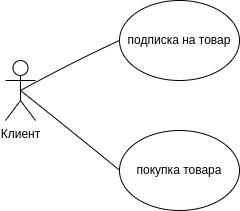
\includegraphics[width=0.6\textwidth]{uml_use_case.png}
	\caption{Варианты использования для работы аптеки}
	\label{fig:use_case}
\end{figure}

\section{Вариант использования "<покупка товара">}
В первую очередь выберем наиболее важный из перечисленных
вариантов использования, включим его в модель анализа, определим для него
классы анализа (классификаторы) и определим отношений между ними.
В качестве наиболее важного варианта использования выберем вариант
"<покупка товара">, в котором участвуют четыре класса (рис. \ref{fig:buy}):
\begin{itemize}
	\item поисковая строка --- граничный класс;
	\item доставка --- граничный класс;
	\item оплата --- управляющий класс;
	\item склад --- класс сущности.
\end{itemize}
\begin{figure}[h!tp]
	\centering
	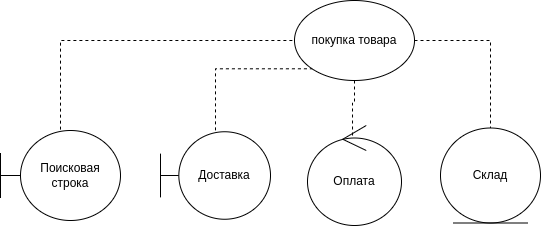
\includegraphics[width=0.8\textwidth]{uml_buy}
	\caption{Состав классов варианта использования "<покупка товара">}
	\label{fig:buy}
\end{figure}

Установим отношения между классами варианта использования
"<покупка товара"> (рис. \ref{fig:buy:impl}).
\begin{figure}[h!tp]
	\centering
	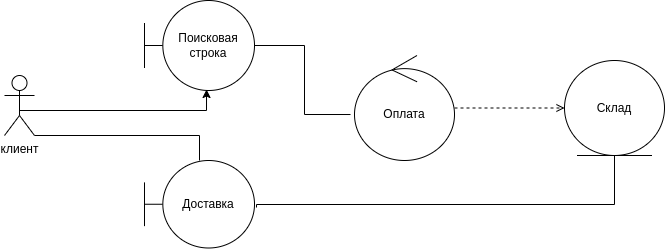
\includegraphics[width=0.8\textwidth]{uml_buy_impl}
	\caption{Реализации варианта использования "<покупка товара">}
	\label{fig:buy:impl}
\end{figure}

\section{Вариант использования "<подписка на товар">}
Повторим первые два шага для варианта использования
«Перечислить деньги на другой счет» (рис. \ref{fig:subscription}),
выделим классы (возможно новые классы анализа) и установим отношения
между ними. В варианте использования "<подписка на товар"> участвуют классы:
\begin{itemize}
	\item личный кабинет пользователя --- граничный класс;
	\item доставка --- граничный класс;
	\item БД пользователей --- класс сущности;
	\item склад --- класс сущности;
	\item оплата --- управляющий класс.
\end{itemize}
\begin{figure}[h!tp]
	\centering
	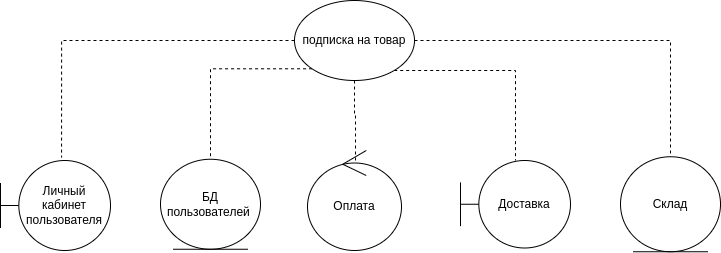
\includegraphics[width=0.8\textwidth]{uml_subscription}
	\caption{Состав классов варианта использования "<подписка на товар">}
	\label{fig:subscription}
\end{figure}

Установим отношения между классами варианта использования "<подписка на товар">
точно также, как и в шаге 2 (рис. \ref{fig:subscription:impl}).
\begin{figure}[h!tp]
	\centering
	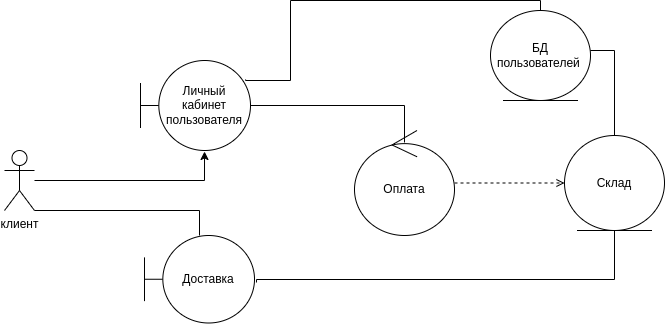
\includegraphics[width=0.8\textwidth]{uml_subscr_impl}
	\caption{Реализации варианта использования "<подписка на товар">}
	\label{fig:subscription:impl}
\end{figure}

\section{Итоговая диаграмма}
Создадим итоговую диаграмму классов анализа (рис. \ref{fig:complite}).
На рисунке видим классы, участвующие в нескольких реализациях варианта
использования модели анализа.
\begin{figure}[h!tp]
	\centering
	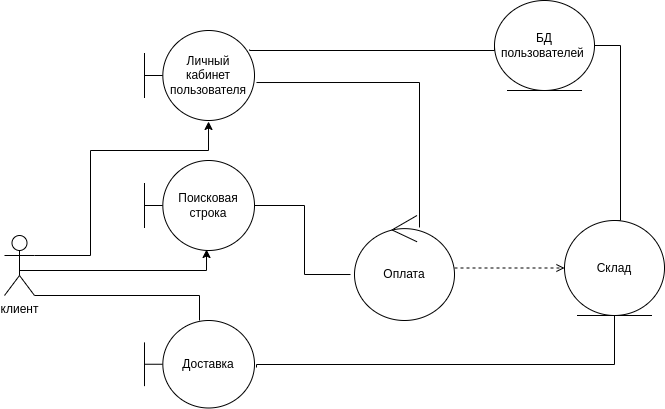
\includegraphics[width=0.8\textwidth]{uml_complite}
	\caption{Реализации варианта использования "<подписка на товар">}
	\label{fig:complite}
\end{figure}

\newpage

\section*{Ответы на вопросы}
\addcontentsline{toc}{section}{Ответы на вопросы}

\begin{enumerate}
	\item \textbf{Перечислите 3 уровня абстракции классов.}\\
		Принято выделять 3 уровня абстракции классов:
		\begin{itemize}
			\item аналитический уровень (концептуальный уровень);
			\item уровень проектирования (уровень спецификации);
			\item уровень реализации (имплементационный уровень).
		\end{itemize}
	\item \textbf{Что собой представляет диаграмма классов
		аналитического уровня?}\\
		\textit{Диаграмма классов анализа} --- это структурная диаграмма языка
		моделирования UML, демонстрирующая общую структуру иерархии классов
		системы, их коопераций, атрибутов, методов, интерфейсов
		и взаимосвязей между ними.
	\item \textbf{Что собой представляет класс анализа?}\\
		\textit{Класс анализа} --- это укрупненная абстракция одного
		или более классов (подсистем в проекте системы),
		которая на концептуальном уровне
		(без 16 точного определения атрибутов и операций)
		описывает некоторый фрагмент системы.
	\item \textbf{Для чего нужна диаграмма классов анализа?}\\
		\textit{Диаграмма классов анализа} необходима как для выявления
		внутренней архитектуры (определения подсистем и основных классов)
		системы, так и для поиска альтернативных вариантов реализации системы
		(подсистемы). На диаграммах классов анализа целесообразно указать
		только наименования классов, атрибуты и операции обычно не указываются
		(хотя можно их только определить), отложив их исследование
		на более поздние стадии детализации.
	\item \textbf{Перечислите стереотипы классов анализа.}\\
		Существует три вида (стереотипа) классов анализа:
		\begin{itemize}
			\item \textit{граничный класс (boundary class)} --- класс,
				который располагается на границе системы с внешней средой
				и непосредственно взаимодействует с актерами, но является
				составной частью системы.
				На диаграмме граничный класс имеет стереотип <<boundary>>;
			\item \textit{класс-сущность (entity class)} --- пассивный класс,
				абстракции основных понятий предметной области,
				хранимых в табличном или ином виде.
				Класс-сущность только принимает сообщения от других классов.
				На диаграмме класс-сущность имеет стереотип <<entity>>;
			\item \textit{управляющий класс (control class)} --- класс,
				который отвечает за координацию действий других классов.
				На диаграмме управляющий класс имеет стереотип <<control>>.
		\end{itemize}
	\item \textbf{Как отображаются классы анализа графически?}\\
		Классы анализа графически отображаются либо в виде классического
		(односекционного) прямоугольника класса с указанием соответствующих
		стереотипов во французских кавычках, либо в виде графических
		примитивов, соответствующих этим видам классов
		(рис.~\ref{fig:analysis_classes}).
		\begin{figure}[h!tp]
			\centering
			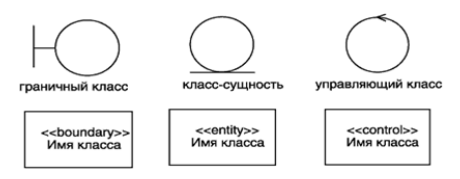
\includegraphics[width=0.8\textwidth]{Screenshot from 2023-03-01 13-33-28}
			\caption{Графическое изображение классов анализа}
			\label{fig:analysis_classes}
		\end{figure}
	\item \textbf{Как могут быть связаны классы анализа?
		Перечислите названия отношений.}\\
		Классы анализа, как элементы системы, естественно связаны между собой
различными отношениями. Используется пяти видов отношений:
		\begin{itemize}
			\item ассоциаций;
			\item агрегаций;
			\item композиций;
			\item наследования;
			\item зависимостей.
		\end{itemize}
	\item \textbf{Что собой представляет отношение ассоциации?}\\
		\textit{Отношение ассоциации} показывает, что объекты одного класса
		содержат информацию о существовании (наличии в памяти) объектов
		другого класса и между ними имеется некоторая логическая
		или семантическая связь.
	\item \textbf{Что собой представляет отношение агрегации?}\\
		\textit{Отношение агрегации} указывает на отношение «часть»-«целое»
		и отображается сплошной линией с незакрашенным ромбиком
		со стороны «целого».
	\item \textbf{Что собой представляет отношение композиции?}\\
		\textit{Отношение композиции} аналогично агрегации, в которой «части»
		не могут существовать отдельно от «целого». При уничтожении
		объекта-«целого» должны быть уничтожены все связанные с ним
		объекты-«части».
	\item \textbf{Что собой представляет отношение наследования (обобщения)?}\\
		\textit{Отношение обобщения (наследования)} является отношением между
		более общим классом и его частным случаем. Отношение обобщения
		может быть только между классами одного вида.
	\item \textbf{Что собой представляет отношение зависимости?}\\
		\textit{Отношение зависимости} означает, что в спецификации
		или теле методов объектов одного класса (зависимого) выполняется
		обращение к атрибутам, методам или непосредственного к объектам
		другого класса (независимого). Графически данное отношение
		обозначается штриховой стрелкой от зависимого класса к независимому
		классу. Данное отношение может указываться между классами анализа
		как одного, так и разных типов.
	\item \textbf{Опишите пошаговый алгоритм создания диаграммы
		классов анализа.}\\
		\textbf{Шаг 1.} Выполнить анализ предметной области,
		используя диаграмму вариантов использования. Выбрать сначала
		наиболее важный из перечисленных вариантов использования для
		включения его в модель анализа, затем по приоритету остальные.\par
		\textbf{Шаг 2.} Определить основные классы анализа для выбранного
		варианта использования (достаточно будет исходного наброска
		наиболее важных для архитектуры системы). Для определения классов
		анализа уточните описание варианта использования в части,
		относящейся к внутреннему строению системы.\par
		\textbf{Шаг 3.} Для каждого найденного класса определить их
		названия, ответственности и отношения.\par
		\textbf{Шаг 4.} Разработать в программной среде модель классов
		анализа, установить между классами соответствующие отношения.
		Шаги 1-4 повторить для каждого варианта использования.\par
		\textbf{Шаг 5.} Создать общую модель классов анализа,
		выполнить идентификацию обязанностей участвующих классов и
		определить отношения между ними. Выполнить исследование отношений
		между найденными классами, используя возможные типы связей,
		уделяя особое внимание классам, участвующим в разных вариантах
		использования и новым классам.\par
		\textbf{Шаг 6.} Сохранить диаграмму, сделать выводы и оформить
		отчет по практической работе.\par
\end{enumerate}

\newpage

\section*{\LARGE Вывод}
\addcontentsline{toc}{section}{Вывод}
В результате практическои работы была создана диаграмма классов анализа,
идентифицированна обязанности участвующих классов анализа и определили
отношения между ними. Доставка, оплата и склад участвуют и
исполняют роли во всех трех реализациях вариантов использования. Видно,
что некоторые из классов могут оказаться новыми или изменившимися ролями
уже обнаруженных классов анализа, в то время как другие роли потребуют
новых классов анализа.\par
При проектировании классов анализа по различным стереотипам требуются
различные навыки и технологии. Так, например, проектирование классов
сущностей обычно требует использования технологий баз данных, в то время
как проектирование граничных классов — использования технологий
пользовательского интерфейса. Однако классы анализа с их ответственностями,
атрибутами и связями используются в качестве (логических) исходных данных
для создания соответствующих операций, атрибутов и отношений классов
проекта.
